\section{The endpoint moved}
\label{sec:endpoint}

Ten and a half hours into a thirty-three hour run, between repetition round 3
(which ended 2026-08-26 06:47 UTC) and round 4 (which began 06:49 UTC), the
results changed character. Nothing changed on our side: same image
digest, same task-set commit, same model identifier, same pinned provider and
quantization, same temperature and seed, same code.

\begin{figure}[t]
\centering
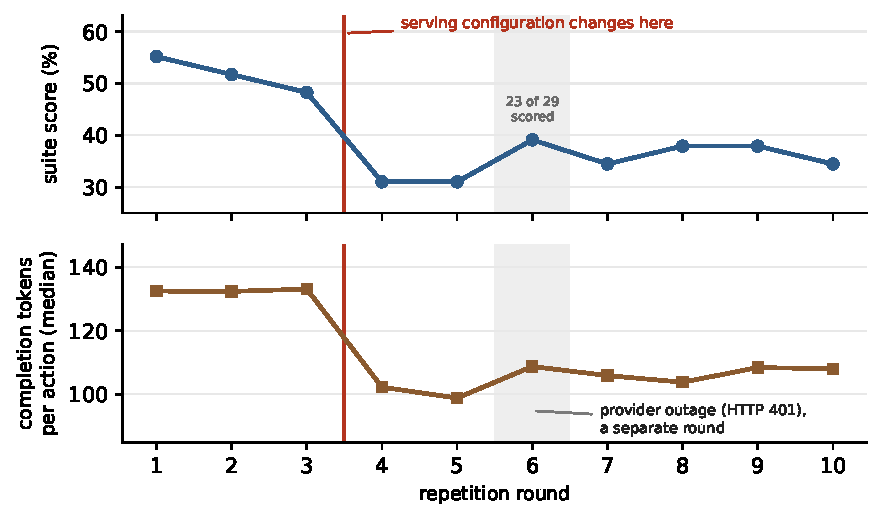
\includegraphics[width=0.80\textwidth]{figures/fig_regime.pdf}
\caption{Suite score and reasoning volume per repetition round, on a shared
axis. Both step at the same place, between rounds 3 and 4 (red line), and both
hold at the new level for the remaining seven rounds. The provider outage
(shaded, round 6) is a separate event at a different round; the step is not the
outage. Round 6 scored 23 of 29 tasks and is annotated accordingly. Two stacked
panels rather than one plot with two vertical axes, so that no choice of scale
can be doing the work.}
\label{fig:regime}
\end{figure}

\subsection{Five checks on the same trajectories, corroborated outside them}

\paragraph{1. Every task that moved, moved the same way.} Ten tasks changed
pass rate across the boundary; all ten got worse, none improved, nineteen were
unchanged. Figure~\ref{fig:dumbbell} shows all ten arrows pointing the same
way, which repetition noise alone would rarely produce: an exact sign test on the
ten gives $p = 0.002$. We read that as an indication of how one-sided the split
is rather than as a hypothesis test at face value, since tasks within a round
share a container, the backend services and an execution order, and so are not
strictly independent.

\begin{figure}[t]
\centering
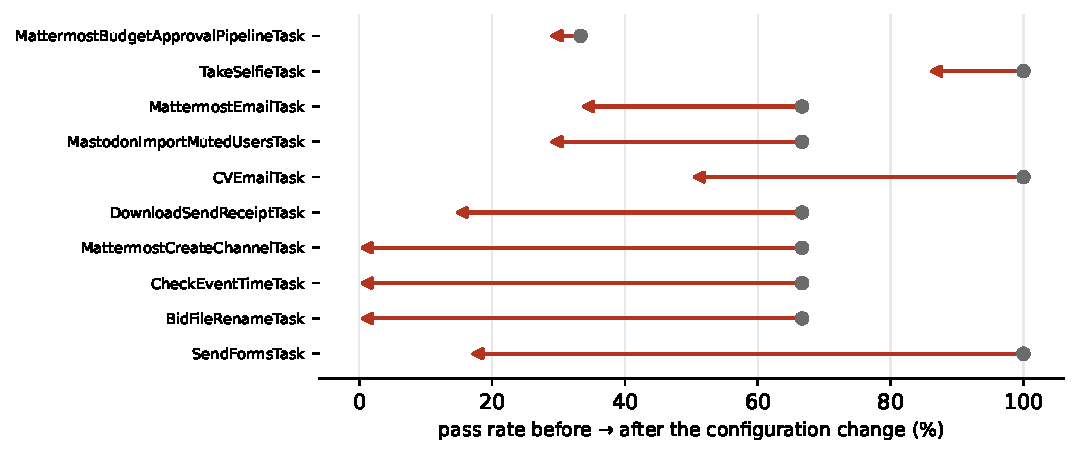
\includegraphics[width=0.86\textwidth]{figures/fig_dumbbell.pdf}
\caption{Per-task pass rate before and after the boundary, one arrow per task
that moved. Ten tasks moved and all ten moved the same way: 10 worse, 0 better,
19 unchanged (exact sign test $p = 0.002$, read as an indication of how
one-sided the split is; tasks within a round are not strictly independent).}
\label{fig:dumbbell}
\end{figure}

\paragraph{2. Reasoning volume stepped, and did not drift.} Median completion
tokens per action --- one step is one model request, and the output is almost
entirely reasoning --- were 132.5, 132.4, 133.1 in rounds 1--3, within 0.55\%
of each other, and 102.2, 98.8, 108.7, 105.9, 103.8, 108.4, 108.0 in rounds
4--10, spanning 98.8--108.7, about $\pm$4.8\% around the regime midpoint.
Between the two regimes the median fell 20.1\%.

\paragraph{3. Faster and worse at the same time.} Comparing rounds 1--3 with
rounds 4--10 throughout (round 6 in, its six zero-step no-verdict runs out):
mean time per step fell from 16.0\,s to 13.7\,s while
quality fell. Degrading hardware or a congested network makes an endpoint
slower, not quicker. Generating less reasoning per call explains both
directions at once, and it explains the third-order effects too: mean steps per
run rose from 28.7 to 30.6 and the share of runs stopped by the 50-step budget
rose from 31\% to 45\%.

\paragraph{Time of day does not explain it.} Co-tenant traffic changes batch
composition --- the mechanism \citet{yuan2025nondeterminism} identify --- so a
diurnal effect is a live alternative. Our own schedule rules it out: rounds
9--10 ran 22:21--04:51 UTC, inside the same overnight window as rounds 1--3
(20:10--06:47 UTC), and stayed at the post-shift level. A daily cycle cannot
produce a step that survives a return to the original hours.

\paragraph{4 and 5. Corroborated outside the harness, with a control.} The
determinism probe of Section~\ref{sec:determinism}, unchanged, sent to the
pinned endpoint on two consecutive days: on the first day the three completions
ranged from 1427 to 2812 tokens (sample SD 761), and on the second day they
came back nearly identical (1344, 1292, 1292; sample SD 30). The same probe
against a second provider serving the same model gave 2963, 1448, 1494 on the
first day and 1938, 1672, 2427 on the second, varying on both days. Each cell
is three requests, so we describe rather than test, and we report sample SD
throughout. The probe locates the change to a day; the round boundary comes
from the harness's internal timing. The harness is not involved in either
measurement, and the change in behaviour was specific to the endpoint we had
pinned rather than to the model, the prompt or our tooling.

\paragraph{What we observed, and what we infer.} We observed an endpoint's
behaviour, not its configuration. A serving-side change is the only explanation
we know of that accounts for all of it at once, but we cannot rule out
explanations we have not thought of, and nothing below depends on the cause.

\subsection{Why this is the finding}

Every one of these controls exists and we set it. There is no flag that pins
how a provider serves the model, because serving behaviour is not part of the
API contract; it is an operational property of somebody else's fleet. And there
is no field in any leaderboard entry, on this board or the others we looked at,
that records which configuration produced the number.

This is not a property of the benchmark we happened to use. Any evaluation
built on hosted inference is exposed to this gap between what the submitter
controls and what determines the number, and the more an agent's behaviour
depends on long reasoning chains, the more exposed it is. We observed one such
change in ten repetitions; we have no measurement of how often they happen,
and nothing here should be read as a claim that they are routine.

\paragraph{A cheap side signal, offered with its limits.} The quantity that
made this visible is completion tokens per action. The harness records
\texttt{total\_tokens}, which is 98.5\% prompt in this workload and moved by
8\% across the change: not enough to notice. Completion tokens per action moved
20.1\% in one step, and a per-round check of the kind our sentinel uses fires
on it at the boundary round while a score test at the same granularity does
not. We call this a side signal, not a detector: it has
worked once, after the fact. A sentinel probe logging fixed requests to 14
endpoints over three weeks raised five length alarms in 328 endpoint-days, none
on two consecutive days; day-shuffled calibration puts the false-alarm rate at
0.06\%. The sentinel measures the output length of fixed requests, a close
relative of tokens per action rather than the same quantity, and a quiet period
calibrates false alarms, not sensitivity. Recording the signal cost nothing
and we had to recover it from raw trajectories after the fact. We recommend
logging it by default (Section~\ref{sec:recs}).
